\documentclass[landscape]{article}
\usepackage{wallpaper}
\usepackage{niceframe}
\usepackage{xcolor}
\usepackage{ulem}
\usepackage{graphicx}
\usepackage{geometry}
\usepackage{polyglossia}
\geometry{tmargin=.5cm,bmargin=.5cm,
lmargin=.5cm,rmargin=.5cm}
\usepackage{multicol}
\setlength{\columnseprule}{0.4pt}
\columnwidth=0.3\textwidth

% Languages
\setmainfont[Language=English]{Source Sans Pro}
\setdefaultlanguage{english}
\setotherlanguages{marathi}
\newfontfamily\marathifont[Mapping=velthuis-sanskrit,Script=Devanagari,Language=Marathi]{Noto Serif Devanagari}
\newcommand \mymarathi[1]{
    \textmarathi{#1}
}
% Languages

\begin{document}

\TileWallPaper{4cm}{2cm}{tiling.png}

\centering
\scalebox{3}{\color{green!30!black!60}
\begin{minipage}{.33\textwidth}
\font\border=umrandb
\generalframe
{\border \char113} % up left
{\border \char109} % up
{\border \char112} % up right
{\border \char108} % left 
{\border \char110} % right
{\border \char114} % lower left
{\border \char111} % bottom
{\border \char115} % lower right
{\centering

\begin{minipage}{.9\textwidth}
\centering

\includegraphics[height=1.5cm]{fls-school-logo.png}
\end{minipage}
\vspace{-8mm}

\curlyframe[.9\columnwidth]{

\textcolor{red!10!black!90}
{\small Free Learner's School, Year 20xx-yy}\\

\textcolor{green!10!black!90}{
\tiny In honor of being generally happy and learning something new}

\smallskip

\textcolor{red!30!black!90}
{\textit{Certificate of}}

\textcolor{black}{\large \textsc{Achievement}}

\vspace{2mm}

\tiny
\uline{
    \textcolor{magenta}{\mymarathi{naava} a.w.a.\footnote{also written as} Name}
}

(Sixth Grade Graduate)

\vspace{4mm}

{\color{blue!40!black}
\scalebox{.7}{
\begin{tabular}{ccccc}
%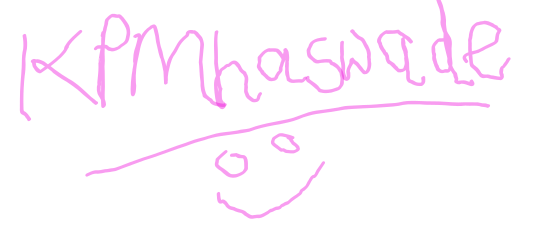
\includegraphics[height=0.4cm]{kedar-sign.png} & & & & 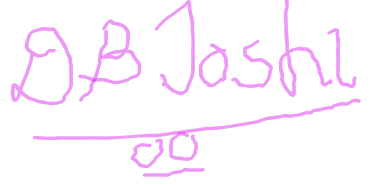
\includegraphics[height=0.4cm]{deepa-sign.png}\\
\cline{1-1} 
%\cline{3-3}
\cline{5-5}
\\
Kedar Mhaswade  & &  & & Deepa Joshi \\
Steacher & & & & Steacher \\ 
\end{tabular}
}}}}
\end{minipage}
}
\end{document}
